\documentclass[
  11pt,
  letterpaper,
   addpoints,
  %answers
  ]{exam}

% Carga el preámbulo localizado en la carpeta superior
\NeedsTeXFormat{LaTeX2e}[2023/04/30]

% Provide the name of your page, the date it was last updated, and a comment about what it's used for
\ProvidesPackage{../exercise-preamble}[2023/04/30 Prof. Cassanelli custom LaTeX style]

% \usepackage{printlen}
% \uselengthunit{in}\printlength{\textwidth}

% PACKAGES
\usepackage[dvipsnames]{xcolor}

\usepackage{graphicx}
\graphicspath{{../figures}}
\usepackage{amsmath,amsthm,amssymb,mathtools,mathrsfs}
\usepackage{commath}
\usepackage{upgreek}
\usepackage{cancel}
\usepackage{enumerate}
\usepackage[font=small]{caption}
\usepackage[normalem]{ulem}
\usepackage{steinmetz}

\usepackage[left=1.5cm, right=1.5cm, top=1cm]{geometry}

% REFERENCES AND OTHERS
\usepackage{../aas_macros}
\usepackage{natbib}
\bibpunct{(}{)}{;}{a}{}{,}

\usepackage{tikz}
\usepackage{tikz-3dplot}
\usepackage{circuitikz}
\usepackage{pgfplots}
\pgfplotsset{compat=1.15}
\usepgfplotslibrary{smithchart}
\usetikzlibrary{
  decorations.pathmorphing,
  decorations.markings,
  calc,
  patterns,
  decorations,
  angles,
  quotes,
  ext.topaths.arcthrough,
  shapes
  }

\usepackage{siunitx}
\sisetup{
    range-phrase=\text{--},
    range-units=single,
    separate-uncertainty=true,
    print-unity-mantissa=false
    }
\DeclareSIUnit{\gauss}{G}
\DeclareSIUnit{\jansky}{Jy}

\newcommand{\iu}{\mathrm{i}\mkern1mu}
\newcommand{\ju}{\mathrm{j}\mkern1mu}
\newcommand{\euler}{\mathrm{e}}
\newcommand{\exponential}[1]{\mathrm{exp}\left[#1\right]}
\newcommand{\uvec}[1]{\widehat{\mathbf{#1}}}
\newcommand{\uvecs}[1]{\boldsymbol{\widehat{#1}}}
\newcommand{\bvec}[1]{\boldsymbol{\mathcal{#1}}}

\usepackage{hyperref}
\hypersetup{
    % bookmarks=true,
    unicode=true,
    pdftoolbar=true,
    pdfmenubar=true,
    pdffitwindow=false,
    pdfstartview={FitH},
    pdftitle={EL3103},
    pdfauthor={Tomas Cassanelli},
    pdfcreator={Tomas Cassanelli},
    pdfnewwindow=true,
    colorlinks=true,
    linkcolor=Violet,
    citecolor=Violet,
    urlcolor=Violet
    }

% Exam document class
\renewcommand{\figurename}{Figura}
\renewcommand{\tablename}{Cuadro}
\pagestyle{empty}

\usepackage[spanish]{cleveref}

\crefname{question}{\protect{pregunta}}{\protect{preguntas}}
\Crefname{question}{\protect{Pregunta}}{\protect{Preguntas}}
\creflabelformat{question}{#2{#1}#3}

\renewcommand{\solutiontitle}{\noindent\textbf{Solución:}\par\noindent}
\bracketedpoints
\pointname{~puntos}

\endinput

% Paquetes locales
\usepackage{float}
\usepackage{booktabs} % para \toprule, \midrule, \bottomrule
\usepackage{xcolor} % para colores
\usepackage{bm} % para negrita en símbolos matemáticos

% Macros locales
\newcommand{\Rel}{\mathfrak{R}} % símbolo para la reluctancia
\DeclareMathOperator{\Var}{Var} % operador de varianza

\begin{document}

% Configuración del encabezado usando comandos de la clase exam
\pagestyle{headandfoot}
\extraheadheight{0.5in} % Baja el encabezado aumentando el espacio superior
\firstpageheader{\textit{Análisis de Sistemas Dinámicos y Estimación}}{}{EL3204-1}
\runningheader{\textit{Análisis de Sistemas Dinámicos y Estimación}}{}{EL3204}
\firstpagefooter{}{\thepage}{}
\runningfooter{}{\thepage}{}
\headrule % Línea debajo del encabezado

% Numeración de página
\pagenumbering{arabic}

% Portada
\begin{center}
    \vspace*{1cm}
    
    % Logo superior
    \includegraphics[width=0.5\textwidth]{../fcfm_die}
    
    \vspace{2cm}
    
    % Líneas decorativas superiores
    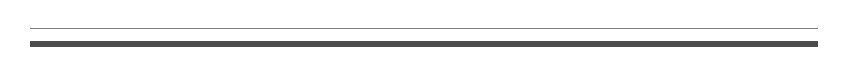
\begin{tikzpicture}
        \draw[line width=2pt, black!70] (0,0) -- (10,0);
        \draw[line width=0.5pt, black!50] (0,0.2) -- (10,0.2);
    \end{tikzpicture}
    
    \vspace{1cm}
    
    % Título principal
    {\fontsize{28}{34}\selectfont\bfseries 
    Análisis de Sistemas\\[0.3cm]
    Dinámicos y Estimación}
    
    \vspace{0.5cm}
    
    {\Large\textbf{EL3204-1}}
    
    \vspace{1cm}
    
    % Líneas decorativas inferiores
    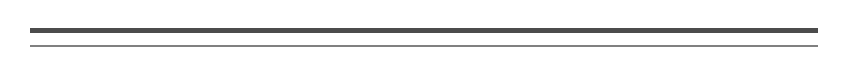
\begin{tikzpicture}
        \draw[line width=0.5pt, black!50] (0,0) -- (10,0);
        \draw[line width=2pt, black!70] (0,0.2) -- (10,0.2);
    \end{tikzpicture}
    
    \vspace{1.5cm}
    
    % Subtítulo
    {\LARGE\itshape Auxiliar 12 - Estimación Bayesiana}
    
    \vspace{0.5cm}
    {\large Prof Marcos Orchard - Sebastian Espinoza.}\\
    {\large Prof Auxiliar Erik Sáez Aravena.}
    
    % Decoración con símbolo matemático de fondo
    \begin{tikzpicture}[remember picture, overlay]
        \node[opacity=0.5, rotate=0] at ([yshift=-8cm]current page.center) {
            \fontsize{280}{300}\selectfont\color{black!15}$\mathcal{I}(\theta)$
        };
    \end{tikzpicture}
    
    \vfill
    
\end{center}

\newpage
%----------------------------
% =========================================
% Unidad III — Estimación de Parámetros (Resumen)
% =========================================
\section*{Resumen}

Este auxiliar cubre conceptos fundamentales de la teoría de estimación de parámetros, que complementa los temas de detección vistos anteriormente. En problemas de detección, el espacio paramétrico $\Theta$ era discreto y finito, pero ahora trabajamos con un conjunto \textbf{infinito no numerable} de posibles valores para el parámetro que queremos estimar (un continuo).

\subsection*{1. Conceptos Básicos de Estimación}
Algunos conceptos importante a considerar son:
\begin{enumerate}
\item \textbf{Espacio de observación ($\mathbb{X}$):} Espacio donde la variable aleatoria $X \in \mathbb{X}$ toma valores. Para vectores aleatorios, $\mathbb{X}^n$ representa el espacio producto.

  \item  \textbf{Espacio de decisión ($\Theta$):} En estimación, es un conjunto \textbf{infinito no numerable} de valores (a diferencia de detección donde era finito). Ejemplos: $\Theta = \mathbb{R}^+$ para estimar amplitudes, $\Theta = \mathbb{R}$ para estimar medias.

\item \textbf{Familia de distribuciones paramétricas ($J_\theta$):} Conjunto de distribuciones indexadas por $\theta$:
\[
J_\theta = \{P_X(x|\theta) : \theta \in \Theta\}
\]

\item \textbf{Estimador:} Una función $\hat{\theta}(x_1, \ldots, x_n)$ que depende de las observaciones y entrega una estimación del parámetro $\theta$ asociado a la distribución $P_X(x|\theta)$.
\end{enumerate}
\subsection*{2. Propiedades de los Estimadores}
\begin{enumerate}
  \item \textbf{Estimador Insesgado:} Un estimador $\hat{\theta}(x_1, \ldots, x_n)$ es insesgado si:
\[
\mathbb{E}[\hat{\theta}(X_1, \ldots, X_n)] = \theta
\]
Es decir, en promedio el estimador entrega el valor verdadero del parámetro.

\item \textbf{Estimador Asintóticamente Insesgado:} Si el sesgo tiende a cero cuando $n \to \infty$:
\[
\lim_{n\to\infty} \mathbb{E}[\hat{\theta}(X_1, \ldots, X_n)] = \theta
\]

\item \textbf{Estimador Consistente:} Un estimador es consistente si converge en probabilidad al valor verdadero:
\[
\lim_{n\to\infty} P_X(|\hat{\theta}(X_1, \ldots, X_n) - \theta| > \epsilon) = 0 \quad \forall \epsilon > 0
\]

\item \textbf{Observación:} Mediante la desigualdad de Chebyshev, si un estimador es insesgado y su varianza tiende a cero cuando $n \to \infty$, entonces es consistente:
\[
\lim_{n\to\infty} \Var(\hat{\theta}(X_1, \ldots, X_n)) = 0 \implies \text{consistencia}
\]
\end{enumerate}
\subsection*{3. Condiciones de Regularidad}

Las condiciones de regularidad permiten intercambiar el orden de derivación e integración en la función de verosimilitud. Bajo estas condiciones se cumple:
\begin{enumerate}
  \item \textbf{Primera condición:} La esperanza de la derivada de la log-verosimilitud es cero:
\[
\mathbb{E}_{X_1^n}\left[\frac{\partial \ln L(X_1, \ldots, X_n|\theta)}{\partial \theta}\right] = 0
\]

\item \textbf{Segunda condición:} La esperanza de un término específico es cero:
\[
\mathbb{E}_{X_1^n}\left[\frac{1}{L(X_1, \ldots, X_n|\theta)}\frac{\partial^2 L(X_1, \ldots, X_n|\theta)}{\partial \theta^2}\right] = 0
\]

\item \textbf{Identidad de Bartlett:} Relaciona la varianza con su segunda derivada:
\[
\mathbb{E}_{X_1^n}\left[\left(\frac{\partial \ln L}{\partial \theta}\right)^2\right] = -\mathbb{E}_{X_1^n}\left[\frac{\partial^2 \ln L}{\partial \theta^2}\right]
\]

Esta identidad permite calcular la información de Fisher de dos formas equivalentes.
\end{enumerate}
\subsection*{4. Información de Fisher}

La información de Fisher $\mathcal{I}(\theta)$ cuantifica cuánta información sobre el parámetro $\theta$ contienen las observaciones:
\[
\mathcal{I}(\theta) = \mathbb{E}\left[\left(\frac{\partial \ln f(X|\theta)}{\partial \theta}\right)^2\right] = -\mathbb{E}\left[\frac{\partial^2 \ln f(X|\theta)}{\partial \theta^2}\right]
\]

\textbf{Propiedad Aditiva:} Para muestras i.i.d., la información de Fisher es aditiva:
\[
\mathcal{I}_n(\theta) = n \cdot \mathcal{I}_1(\theta)
\]

Esta propiedad refleja que más observaciones independientes proporcionan más información sobre el parámetro.

\subsection*{5. Cota de Cramér-Rao}

La cota de Cramér-Rao establece un límite inferior para la varianza de cualquier estimador insesgado:
\[
\Var(\hat{\theta}) \geq \frac{1}{\mathcal{I}(\theta)}
\]
\begin{enumerate}
  \item \textbf{Estimador Eficiente:} Un estimador insesgado que alcanza la cota de Cramér-Rao se llama \textbf{eficiente} o \textbf{de mínima varianza}

\item \textbf{Interpretación:} La información de Fisher es inversamente proporcional a la mínima varianza posible. Más información $\implies$ menor varianza mínima.
\end{enumerate}
\subsection*{6. Estimador de Máxima Verosimilitud (ML)}

El estimador de máxima verosimilitud se obtiene maximizando la función de verosimilitud:
\[
\hat{\theta}_{ML} = \arg\max_{\theta} L(x_1, \ldots, x_n|\theta) = \arg\max_{\theta} \ln L(x_1, \ldots, x_n|\theta)
\]

\textbf{Método de solución:} Criterio de la primera derivada:
\[
\frac{\partial \ln L(x_1, \ldots, x_n|\theta)}{\partial \theta}\bigg|_{\theta=\hat{\theta}_{ML}} = 0
\]

Verificar que la segunda derivada es negativa para confirmar que es un máximo.

\subsection*{7. Estimación Bayesiana}

En el enfoque bayesiano, el parámetro $\theta$ es considerado como una variable aleatoria con una distribución a priori $P_{\Theta}(\theta)$ o $f_{\Theta}(\theta)$. Se busca encontrar estimadores basados en la distribución a posteriori:
\[
f_{\Theta|X}(\theta|x) = \frac{f_{X|\Theta}(x|\theta) f_{\Theta}(\theta)}{f_X(x)}
\]
\begin{itemize}
\item \textbf{Estimador MMSE (Minimum Mean Square Error):}

El estimador que minimiza el error cuadrático medio es la esperanza condicional:
\[
\hat{\theta}_{MMSE}(x) = \mathbb{E}[\Theta|X=x] = \int_{-\infty}^{\infty} \theta \cdot f_{\Theta|X}(\theta|x) d\theta
\]

Para el caso discreto:
\[
\hat{\theta}_{MMSE}(x) = \sum_{\theta} \theta \cdot P_{\Theta|X}(\theta|x)
\]

\item \textbf{Estimador MAP (Maximum A Posteriori):}

El estimador MAP maximiza la distribución a posteriori:
\[
\hat{\theta}_{MAP}(x) = \arg\max_{\theta} f_{\Theta|X}(\theta|x) = \arg\max_{\theta} f_{X|\Theta}(x|\theta) f_{\Theta}(\theta)
\]

Para el caso discreto:
\[
\hat{\theta}_{MAP}(x) = \arg\max_{\theta} P_{\Theta|X}(\theta|x) = \arg\max_{\theta} P_{X|\Theta}(x|\theta) P_{\Theta}(\theta)
\]

En la práctica se trabaja con el logaritmo:
\[
\hat{\theta}_{MAP}(x) = \arg\max_{\theta} \ln f_{X|\Theta}(x|\theta) + \ln f_{\Theta}(\theta)
\]
\end{itemize}

%----------------------------
\newpage
\begin{questions}
\question
\label{q:estimador_exponencial}
Considere el problema de estimar $\theta \in \mathbb{R}$ dada una observación $X \in \mathbb{R}$, se sabe que la distribución condicional de $\Theta$ dado $X$ está dotada de la siguiente función de densidad condicional definida como:
\[
f_{\Theta|X}(\theta|x) = \begin{cases}
e^{-(\theta-x)}, & \text{si } \theta > x \\
0, & \text{si } x > \theta
\end{cases}
\]

Encuentre el estimador de mínimo error cuadrático medio y MAP.

\begin{solution}
  Buscamos obtener los estimadores MMSE y MAP dados los datos del problema. Tenemos la distribución a posteriori $f_{\Theta|X}(\theta|x)$ y debemos encontrar dos estimadores distintos.

\begin{itemize}
\item \textbf{Estimador de Mínimo Error Cuadrático Medio (MMSE):}

Recordemos que el estimador MMSE corresponde a la esperanza condicional:
\[
\hat{\theta}_{MMSE}(x) = \mathbb{E}[\Theta|X=x] = \int_{-\infty}^{\infty} \theta \cdot f_{\Theta|X}(\theta|x) d\theta
\]
Pero tenemos que conocemos función de densidad $f_{\Theta|X}(\theta|x)$, la cual es:
\[
f_{\Theta|X}(\theta|x) = \begin{cases}
e^{-(\theta-x)}, & \text{si } \theta > x \\
0, & \text{si } \theta \leq x
\end{cases}
\]
Entonces, la integral se reduce a:srrrter
\[
\hat{\theta}_{MMSE}(x) = \int_{x}^{\infty} \theta \cdot e^{-(\theta-x)} d\theta
\]

Es conveniente el realizar un cambio de variable $u = \theta - x$, entonces, tendremos que $\theta = u + x$ y $d\theta = du$. Sustituyendo en la integral:
\[
\hat{\theta}_{MMSE}(x) = \int_{0}^{\infty} (u + x) e^{-u} du
\]

Separamos la integral en dos términos:
\begin{align*}
\hat{\theta}_{MMSE}(x) &= \underbrace{\int_{0}^{\infty} u \cdot e^{-u} du}_{1} + \int_{0}^{\infty} x \cdot e^{-u} du \\
&= \underbrace{\int_{0}^{\infty} u \cdot e^{-u} du}_{2} + x \cdot \underbrace{\int_{0}^{\infty} e^{-u} du}_{1}
\end{align*}

Ahora calculamos cada integral por separado por lo que la primera integral sera:
\[
\int_{0}^{\infty} e^{-u} du = \left[-e^{-u}\right]_{0}^{\infty} = \lim_{u \to \infty}(-e^{-u}) - (-e^{0}) = 0 - (-1) = 1
\]
Luego para la segunda integral usaremos integración por partes. Para esto utilizaremos que $\int v \, dw = vw - \int w \, dv$. Para esto consideramos que:
\begin{itemize}
\item $v = u \implies dv = du$
\item $dw = e^{-u}du \implies w = -e^{-u}$
\end{itemize}
Luego,
\begin{align*}
\int_{0}^{\infty} u \cdot e^{-u} du &= \left[u \cdot (-e^{-u})\right]_{0}^{\infty} - \int_{0}^{\infty} (-e^{-u}) du\\
&= \left[-u \cdot e^{-u}\right]_{0}^{\infty} + \int_{0}^{\infty} e^{-u} du
\end{align*}

Evaluamos el primer término:
\[
\left[-u \cdot e^{-u}\right]_{0}^{\infty} = \lim_{u \to \infty}\left(-u \cdot e^{-u}\right) - (0 \cdot e^{0}) = 0 - 0 = 0
\]

Donde tenemos que  $\lim_{u \to \infty} u \cdot e^{-u} = 0$ porque la exponencial decrece más rápido que $u$ crece. El segundo término ya lo calculamos antes y vale $1$. 
\[
\int_{0}^{\infty} u \cdot e^{-u} du = 0 + 1 = 1
\]
Luego tenemos que combinando las integrales, se tendra que:
\[
\hat{\theta}_{MMSE}(x) = \int_{0}^{\infty} u \cdot e^{-u} du + x \cdot \int_{0}^{\infty} e^{-u} du = 1 + x \cdot 1 = x + 1
\]

Por lo tanto, el estimador MMSE es:
\[
\boxed{\hat{\theta}_{MMSE}(x) = x + 1}
\]

\item \textbf{Estimador MAP (Maximum A Posteriori)}:

El estimador MAP maximiza la densidad a posteriori:
\[
\hat{\theta}_{MAP}(x) = \arg\max_{\theta} f_{\Theta|X}(\theta|x)
\]

Recordemos que la función de densidad es:
\[
f_{\Theta|X}(\theta|x) = \begin{cases}
e^{-(\theta-x)}, & \text{si } \theta > x \\
0, & \text{si } \theta \leq x
\end{cases}
\]
Para encontrar el máximo, analizamos el comportamiento de $f_{\Theta|X}(\theta|x) = e^{-(\theta-x)}$ en la región donde $\theta > x$. Calculamos la derivada con respecto a $\theta$:
\[
\frac{d}{d\theta} f_{\Theta|X}(\theta|x) = \frac{d}{d\theta} e^{-(\theta-x)} = -e^{-(\theta-x)}
\]

Como $e^{-(\theta-x)} > 0$ para todo $\theta$, tenemos que:
\[
\frac{d}{d\theta} f_{\Theta|X}(\theta|x) = -e^{-(\theta-x)} < 0 \quad \text{para todo } \theta > x
\]

La derivada es siempre negativa en la región donde la función está definida, lo que significa que $f_{\Theta|X}(\theta|x)$ es una función estrictamente decreciente. Por lo tanto, el máximo de $f_{\Theta|X}(\theta|x)$ se alcanza en el valor más pequeño posible de $\theta$, que es $\theta = x$ 
Evaluando en ese punto:
\[
f_{\Theta|X}(x|x) = e^{-(x-x)} = e^0 = 1
\]

Y para cualquier $\theta > x$:
\[
f_{\Theta|X}(\theta|x) = e^{-(\theta-x)} < 1
\]

Concluimos que el estimador MAP es:
\[
\boxed{\hat{\theta}_{MAP}(x) = x}
\]

Otra forma de realizar el análisis es mediante el uso del logaritmo de la función de densidad a posteriori. El estimador MAP maximiza:
\begin{align*}
\hat{\theta}_{MAP}(x) &= \arg\max_{\theta} \ln[f_{\Theta|X}(\theta|x)]\\
&= \arg\max_{\theta} \ln[e^{-(\theta-x)}] \\
&= \arg\max_{\theta} (-(\theta - x)) \\
&= \arg\max_{\theta} (x - \theta)
\end{align*}

Ahora, para encontrar el máximo de $g(\theta) = x - \theta$ en la región $\theta > x$, aplicamos el criterio de la primera derivada:
\[
\frac{d}{d\theta}(x - \theta) = -1 < 0
\]

Como la derivada es constante y negativa, la función $g(\theta) = x - \theta$ es estrictamente decreciente en $\theta$. Por lo tanto, el máximo se alcanza en el menor valor posible de $\theta$ en la región donde está definida, es decir, en el límite inferior $\theta = x$. Con lo que podemos confirmar nuevamente que:
\[
\boxed{\hat{\theta}_{MAP}(x) = x}
\]

\begin{itemize}
\item El estimador MAP $\hat{\theta}_{MAP}(x) = x$ elige el valor que maximiza la probabilidad a posteriori.
\item El estimador MMSE $\hat{\theta}_{MMSE}(x) = x + 1$ considera toda la distribución a posteriori y minimiza el error cuadrático medio esperado.
\end{itemize}
\end{itemize}
\end{solution}

\question
\label{q:estimador_normal_bayesiano}
Sean $X_1, \ldots, X_n$ muestras i.i.d. de la variable aleatoria $X \sim \mathcal{N}(\mu, \sigma^2)$. A su vez, $\mu$ es una variable aleatoria continua tal que $\mu \sim \mathcal{N}(0, \sigma_0^2)$.

\begin{enumerate}
\item Determine las densidades $f_{X_1, \ldots, X_n}(x_1, \ldots, x_n|\mu)$ y $f_{M}(\mu)$.
  \begin{solution}

Dado que nos pide el estimador MAP de $\mu$, debemos encontrar la densidad conjunta condicional de las muestras $X_1, \ldots, X_n$ dado $\mu$ y la densidad de $\mu$. Luego, usaremos estas densidades para encontrar el estimador MAP. Como se ha visto en auxiliares anteriores, se tiene la siguiente densidad conjunta condicional para el vector $X$:
\begin{align*}
f_X(x_1, \ldots, x_n|\mu) = \prod_{i=1}^{n} f_{X_i}(x|\mu) &= \prod_{i=1}^{n} \frac{1}{\sqrt{2\pi\sigma^2}} \cdot exp\left(-\frac{(x_i-\mu)^2}{2\sigma^2}\right) \\
&= \left(\frac{1}{2\pi\sigma^2}\right)^{\frac{n}{2}} \cdot exp\left(-\frac{1}{2\sigma^2}\sum_{i=1}^{n}(x_i-\mu)^2\right)
\end{align*}
Por otro lado, la densidad de la variable aleatoria $M = \mu$ es una normal conocida:
\[
f_{M}(\mu) = \frac{1}{\sqrt{2\pi\sigma_0^2}} \cdot e^{-\frac{\mu^2}{2\sigma_0^2}}
\]
Con lo que tenemos las densidades buscadas.
  \end{solution} 

\item Obtenga el estimador MAP de $\mu$, $\hat{\mu}_{MAP}$.

\begin{solution}
Por definición, se tiene que el estimador MAP es:
\begin{align*}
\hat{\mu}_{MAP} &= \arg\max_{\mu} f_{\mu|X}(\mu|x_1, \ldots, x_n)
\end{align*}
Luego tenemos que por teorema de Bayes:
\begin{align*}
f_{\mu|X}(\mu|x_1, \ldots, x_n) &= \frac{f_X(x_1, \ldots, x_n|\mu) \cdot f_{\mu}(\mu)}{f_X(x_1, \ldots, x_n)}
\end{align*}
Como el denominador no depende de $\mu$, podemos ignorarlo en la maximización. Por lo tanto, el estimador MAP se puede expresar como:
\[
\hat{\mu}_{MAP} = \arg\max_{\mu} \ln[f_X(x_1, \ldots, x_n|\mu) \cdot f_{\mu}(\mu)]
\]

Obtengamos la expresión a maximizar:
\begin{align*}
\ln[f_X(x_1, \ldots, x_n|\mu) \cdot f_{\mu}(\mu)] = &= \ln\left[\left(\frac{1}{2\pi\sigma^2}\right)^{\frac{n}{2}} \cdot exp\left(-\frac{1}{2\sigma^2}\sum_{i=1}^{n}(x_i-\mu)^2\right) \cdot \frac{1}{\sqrt{2\pi\sigma_0^2}} \cdot e^{-\frac{\mu^2}{2\sigma_0^2}}\right] \\
&= -\frac{n}{2}\ln(2\pi\sigma^2) - \frac{1}{2\sigma^2} \cdot \sum_{i=1}^{n}(x_i - \mu)^2 - \frac{1}{2}\ln(2\pi\sigma_0^2) - \frac{\mu^2}{2\sigma_0^2}
\end{align*}

Luego, aplicamos el criterio de la primera derivada para lo cual asumimos que obtendremos un máximo (se puede verificar con la segunda derivada que efectivamente es un máximo):
\begin{align*}
\frac{d}{d\mu}\left(\cancel{-\frac{n}{2}\ln(2\pi\sigma^2)} - \frac{1}{2\sigma^2} \cdot \sum_{i=1}^{n}(x_i - \mu)^2 \cancel{- \frac{1}{2}\ln(2\pi\sigma_0^2)} - \frac{\mu^2}{2\sigma_0^2}\right) &= 0 \\
 - \frac{1}{2\sigma^2} \cdot \sum_{i=1}^{n}\frac{d}{d\mu}(x_i - \mu)^2 - \frac{1}{2\sigma_0^2}\frac{d}{d\mu}\mu^2 &= 0 \\
- \frac{1}{2\sigma^2} \cdot \sum_{i=1}^{n}2(x_i - \mu)(-1) - \frac{1}{2\sigma_0^2}(2\mu) &= 0 \\
\frac{1}{\sigma^2} \cdot \sum_{i=1}^{n}(x_i - \mu) - \frac{\mu}{\sigma_0^2} &= 0 \\
\frac{1}{\sigma^2}\sum_{i=1}^{n}x_i - \frac{n\mu}{\sigma^2} - \frac{\mu}{\sigma_0^2} &= 0 \\
\frac{\sum_{i=1}^{n}x_i}{\sigma^2} &= \mu \cdot \left(\frac{1}{\sigma_0^2} + \frac{n}{\sigma^2}\right) \\
\mu &= \frac{\sum_{i=1}^{n}x_i}{\sigma^2 \cdot \left(\frac{1}{\sigma_0^2} + \frac{n}{\sigma^2}\right)} \\
\mu &= \frac{\sum_{i=1}^{n}x_i}{\left(\frac{\sigma^2}{\sigma_0^2} + n\right)} \\
\mu &= \frac{\sigma_0^2}{n\sigma_0^2 + \sigma^2} \cdot \sum_{i=1}^{n}x_i \\
\mu &= \frac{\sigma_0^2}{\sigma_0^2 + \frac{\sigma^2}{n}} \cdot \frac{1}{n} \cdot \sum_{i=1}^{n}x_i
\end{align*}

Con lo que finalmente el estimador MAP de $\mu$ corresponde a:
\[
\boxed{\hat{\mu}_{MAP} = \frac{\sigma_0^2}{\sigma_0^2 + \frac{\sigma^2}{n}} \cdot \frac{1}{n} \cdot \sum_{i=1}^{n}x_i}
\]
\end{solution}

\item Determine los casos límite en que $\sigma_0^2 \longrightarrow \infty$ y $\sigma_0^2 \longrightarrow 0$. Interprete cada situación.
\end{enumerate}

\begin{solution}
Luego buscamos analizar los casos limites en relacion al parametro $\sigma_0^2$ el cual corresponde a la varianza de la distribución a priori de $\mu$. Analizaremos cada caso por separado:

\begin{itemize}
\item $\sigma_0^2 \longrightarrow \infty$: En este caso tenemos que ver el límite del estimador. Para calcular este límite, dividimos numerador y denominador por $\sigma_0^2$:
\begin{align*}
\lim_{\sigma_0^2 \to \infty} \frac{\sigma_0^2}{\sigma_0^2 + \frac{\sigma^2}{n}} \cdot \frac{1}{n} \cdot \sum_{i=1}^{n}x_i &= \lim_{\sigma_0^2 \to \infty} \frac{\frac{\sigma_0^2}{\sigma_0^2}}{\frac{\sigma_0^2}{\sigma_0^2} + \frac{\sigma^2}{n\sigma_0^2}} \cdot \frac{1}{n} \cdot \sum_{i=1}^{n}x_i \\
&= \lim_{\sigma_0^2 \to \infty} \frac{1}{1 + \frac{\sigma^2}{n\sigma_0^2}} \cdot \frac{1}{n} \cdot \sum_{i=1}^{n}x_i \\
&= \frac{1}{1 + \lim_{\sigma_0^2 \to \infty}\frac{\sigma^2}{n\sigma_0^2}} \cdot \frac{1}{n} \cdot \sum_{i=1}^{n}x_i \\
&= \frac{1}{1 + 0} \cdot \frac{1}{n} \cdot \sum_{i=1}^{n}x_i \\
&= \frac{1}{n} \cdot \sum_{i=1}^{n}x_i
\end{align*}

Podemos notar de este caso que, mientras más incerteza tenemos sobre el parámetro $\mu$ en su distribución (equivalente a que la varianza de la normal sea muy grande), el estimador MAP tiende a la media empírica de las observaciones, es decir, los datos son los que determinan el estimador (Porque le creemos más a los datos que al conocimiento a priori). A su vez corresponde al estimador de máxima verosimilitud del problema.

\item $\sigma_0^2 \longrightarrow 0$: En este caso tenemos que ver el límite del estimador. Para evaluar este límite, multiplicamos numerador y denominador por $n$ y luego aplicamos el límite directamente:
\begin{align*}
\lim_{\sigma_0^2 \to 0} \frac{\sigma_0^2}{\sigma_0^2 + \frac{\sigma^2}{n}} \cdot \frac{1}{n} \cdot \sum_{i=1}^{n}x_i &= \lim_{\sigma_0^2 \to 0} \frac{n\sigma_0^2}{n\sigma_0^2 + \sigma^2} \cdot \frac{1}{n} \cdot \sum_{i=1}^{n}x_i \\
&= \frac{n \cdot 0}{n \cdot 0 + \sigma^2} \cdot \frac{1}{n} \cdot \sum_{i=1}^{n}x_i \\
&= \frac{0}{\sigma^2} \cdot \frac{1}{n} \cdot \sum_{i=1}^{n}x_i \\
&= 0
\end{align*}

En este caso ocurre que tenemos mucha certeza sobre el valor del parámetro $\mu$ en su distribución a priori, lo cual se modela como $\sigma_0^2 \longrightarrow 0$. Cuando la varianza a priori tiende a cero, significa que estamos completamente seguros de que $\mu = 0$ (su esperanza a priori). Por lo tanto, el estimador MAP ignora completamente las observaciones y simplemente devuelve el valor sobre el cual tenemos certeza total: $\hat{\mu}_{MAP} = 0$.  Este resultado tiene sentido intuitivo dado que si estamos absolutamente seguros (varianza cero) de que $\mu = 0$, ninguna cantidad de datos podrá cambiar esta creencia a priori, y el estimador MAP reflejará esta certeza ignorando las mediciones.
\end{itemize}
\end{solution}

\question
\label{q:particulas_radiactivas}
Considere que tiene un cuerpo radiactivo que, dentro de un cierto intervalo de tiempo, emite un cierto $\Theta \in \mathbb{N}$ partículas el cual usted quiere medir con un instrumento el cual le indica el total de partículas detectadas durante dicho intervalo. Sin embargo, su detector es imperfecto, por lo que hay una probabilidad $p$ de que detecte correctamente cada partícula.

Gracias a estudios anteriores, usted sabe que $\Theta \sim \text{Poisson}(\lambda)$, donde $\lambda$ es la propiedad asociada a la tasa de emisión del cuerpo.

\begin{enumerate}
\item Plantee el problema de estimar el número de partículas emitidas a partir del número de partículas detectadas, e indique las distribuciones asociadas. ¿Es un problema de estimación o detección?

\begin{solution}
Para modelar el problema, si se emiten $\Theta \sim \text{Poisson}(\lambda)$ partículas entonces consideremos $\mathbf{B} = (B_1, \ldots, B_{\Theta}) \in \{0,1\}^{\Theta}$, donde $B_i \sim \text{Bernoulli}(p)$ son las variables independientes que indican si la $i$-ésima partícula fue detectada o no. Luego, consideremos
\[
X := \sum_{i=1}^{\Theta} B_i
\]
la medición realizada, correspondiente al número partículas detectadas. De este modo, podemos ver que $X \sim \text{Binom}(\Theta, p)$, por lo que $X|\Theta = \theta \sim \text{Binom}(\theta, p)$. De esta manera podemos definir las siguientes distribuciones asociadas al problema:
\begin{itemize}
\item \textbf{Distribución a priori:} $\Theta \sim \text{Poisson}(\lambda)$ la cual esta asociada al número de partículas emitidas, es decir:
\[
P_{\Theta}(\theta) = \frac{e^{-\lambda}\lambda^{\theta}}{\theta!}, \quad \theta \in \mathbb{N}
\]

\item \textbf{Distribución condicional (verosimilitud) :} $X|\Theta = \theta \sim \text{Binom}(\theta, p)$, la cual esta asociada a la probabilidad de detectar $x$ partículas dado que se emitieron $\theta$, es decir:
\[
P_{X|\Theta}(x|\theta) = \binom{\theta}{x}p^x(1-p)^{\theta-x}, \quad x \in \{0, 1, \ldots, \theta\}
\]

\end{itemize}
Queremos estimar $\Theta$ (número de partículas emitidas) a partir de la observación $X$ (número de partículas detectadas). El objetivo es encontrar un estimador $\hat{\theta}(x)$ que minimice algún criterio de desempeño (por ejemplo, error cuadrático medio para MMSE, o maximice la probabilidad a posteriori para MAP). Formalmente, este es un \textbf{problema de detección}, ya que el espacio de decisión $\Theta \in \mathbb{N}$ es discreto y numerable. Sin embargo, como veremos en las partes siguientes, al relajar el espacio de decisión a los números reales $\mathbb{R}^+$, podemos tratarlo como un problema de estimación, lo cual es útil en la práctica cuando los estimadores óptimos (como el MMSE) entregan valores no enteros.
\end{solution}
\item Encuentre el estimador MMSE.
\begin{solution}

Sabemos que el estimador MMSE $\hat{\theta}_{MMSE}(x)$ por definición está dado por
\[
\hat{\theta}_{MMSE}(x) = \mathbb{E}\{\Theta|X = x\},
\]
por lo que para encontrarlo necesitamos expresar la distribución a posteriori. Para esto, notemos que por Bayes
\[
P_{\Theta|X}(\theta|x) = \frac{P_{X|\Theta}(x|\theta)P_{\Theta}(\theta)}{P_X(x)},
\]
donde
\[
P_{X|\Theta}(x|\theta) = \binom{\theta}{x}p^x(1-p)^{\theta-x}, \quad P_{\Theta}(\theta) = \frac{e^{-\lambda}\lambda^{\theta}}{\theta!}.
\]

A diferencia de lo que hicimos con el estimador MAP de omitir el término del denominador ahora no es posible, por lo que aplicamos la \textbf{ley de probabilidades totales}, que nos dice que para calcular la probabilidad marginal de $X$ debemos sumar sobre todos los posibles valores de $\Theta$. Recodemos que por definicion tenemos que las probabiliades totales es:
\[
P_X(x) = \sum_{\theta \in \mathbb{N}} P_{X|\Theta}(x|\theta)P_{\Theta}(\theta) = \sum_{\theta \geq 0} P_{X|\Theta}(x|\theta)P_{\Theta}(\theta)
\]

Ahora bien, recordemos que $X|\Theta$ sigue una distribución binomial, donde $X$ representa el número de éxitos (partículas detectadas) en $\theta$ intentos. Por la naturaleza de la binomial, es imposible obtener más éxitos que intentos, es decir, $X \leq \Theta$. Esto significa que:
\[
P_{X|\Theta}(x|\theta) = \binom{\theta}{x}p^x(1-p)^{\theta-x} = 0 \quad \text{si } \theta < x
\]

porque el coeficiente binomial $\binom{\theta}{x} = \frac{\theta!}{x!(\theta-x)!}$ no está definido (o es cero) cuando $\theta < x$ (ya que $(\theta-x)!$ sería el factorial de un número negativo, que no existe). Por lo tanto, todos los términos con $\theta < x$ no contribuyen a la suma, y podemos escribir:
{\allowdisplaybreaks
\begin{align*}
P_X(x) &= \sum_{\theta \geq 0} P_{X|\Theta}(x|\theta)P_{\Theta}(\theta)\\ 
&= \sum_{\theta \geq x} P_{X|\Theta}(x|\theta)P_{\Theta}(\theta) \\
&= \sum_{\theta \geq x} \binom{\theta}{x}p^x(1-p)^{\theta-x}\frac{e^{-\lambda}\lambda^{\theta}}{\theta!}\\ 
&= \sum_{\theta \geq x} \frac{1}{x!(\theta-x)!}p^x(1-p)^{\theta-x}e^{-\lambda}\lambda^{\theta} \\
&= \frac{e^{-\lambda}p^x}{x!} \sum_{\theta \geq x} \frac{(\lambda(1-p))^{\theta-x}}{(\theta-x)!} = \frac{e^{-\lambda}(\lambda p)^x}{x!} \sum_{i \geq 0} \frac{(\lambda(1-p))^{i}}{i!}\\ 
&= \frac{e^{-\lambda p}(\lambda p)^x}{x!}
\end{align*}}
Volviendo sobre la distribución a posteriori, tenemos entonces que:
{\allowdisplaybreaks
\begin{align*}
P_{\Theta|X}(\theta|x) &= \frac{P_{X|\Theta}(x|\theta)P_{\Theta}(\theta)}{P_X(x)} = \frac{\binom{\theta}{x}p^x(1-p)^{\theta-x} \cdot \frac{e^{-\lambda}\lambda^{\theta}}{\theta!}}{\frac{e^{-\lambda p}(\lambda p)^x}{x!}} = \frac{\frac{1}{x!(\theta-x)!}p^x(1-p)^{\theta-x} \cdot e^{-\lambda}\lambda^{\theta}}{\frac{e^{-\lambda p}(\lambda p)^x}{x!}} \\
&= \frac{x!}{x!} \cdot \frac{e^{-\lambda}}{e^{-\lambda p}} \cdot \frac{p^x}{(\lambda p)^x} \cdot \frac{\lambda^{\theta}(1-p)^{\theta-x}}{(\theta-x)!} = e^{-\lambda(1-p)} \cdot \frac{\lambda^{\theta-x}(1-p)^{\theta-x}}{(\theta-x)!} = \frac{e^{-\lambda(1-p)}(\lambda(1-p))^{\theta-x}}{(\theta-x)!}
\end{align*}}
Luego, calculando la esperanza tenemos
\begin{align*}
\hat{\theta}_{MMSE}(x) &= \mathbb{E}\{\Theta|X = x\} \\
&= \sum_{\theta \geq x} \theta \cdot P_{\Theta|X}(\theta|x) \\
&= \sum_{\theta \geq x} \theta \cdot \frac{e^{-\lambda(1-p)}(\lambda(1-p))^{\theta-x}}{(\theta-x)!} \qquad / \; i = \theta - x \\
&= e^{-\lambda(1-p)} \sum_{i \geq 0} (i+x) \frac{(\lambda(1-p))^i}{i!} \\
&= e^{-\lambda(1-p)} \left[\sum_{i \geq 0} i \frac{(\lambda(1-p))^i}{i!} + x \sum_{i \geq 0} \frac{(\lambda(1-p))^i}{i!}\right].\\
&= e^{-\lambda(1-p)} \left[\sum_{i \geq 0} i \frac{(\lambda(1-p))^i}{i!} + x\cdot e^{\lambda(1-p)}\right].\\
&= e^{-\lambda(1-p)} \left[\sum_{i \geq 0} i \frac{(\lambda(1-p))^i}{i(i-1)!} + x\cdot e^{\lambda(1-p)}\right].\\
&= e^{-\lambda(1-p)} \left[\sum_{i \geq 0} \frac{(\lambda(1-p))^i}{(i-1)!} + x\cdot e^{\lambda(1-p)}\right].\\
&= e^{-\lambda(1-p)} \left[\sum_{i \geq 0} \frac{(\lambda(1-p))^{j+1}}{(j)!} + x\cdot e^{\lambda(1-p)}\right].\\
&= e^{-\lambda(1-p)} \left[\lambda(1-p) \sum_{j \geq 0} \frac{(\lambda(1-p))^{j}}{(j)!} + x\cdot e^{\lambda(1-p)}\right].\\
&= e^{-\lambda(1-p)} \left[\lambda(1-p) \cdot e^{\lambda(1-p)} + x \cdot e^{\lambda(1-p)}\right].\\
&= e^{-\lambda(1-p)} \cdot e^{\lambda(1-p)} \left[\lambda(1-p) + x\right].\\
&= \lambda(1-p) + x \\
&= x + \lambda(1-p),
\end{align*}
de modo que el estimador MMSE está dado por
\[
\boxed{\hat{\theta}_{MMSE}(x) = x + \lambda(1-p).}
\]

Podemos ver que, pese a que $\Theta \in \mathcal{A} = \mathbb{N}$ (es decir, el problema es de detección), dado que $\lambda \in \mathbb{R}^+$ y $p \in (0,1)$ el estimador elige valores dentro de $\mathbb{R}^+$, y por lo tanto el problema se trata, indirectamente, como uno de estimación.
\end{solution}
\item Encuentre el estimador MAP, relajando el espacio de decisión a los números reales. \textit{Indicación:} Considere que $\Gamma(z+1) = z!$ es la continuación analítica de los factoriales, y que $\psi(z) = \frac{d\log\Gamma(z)}{dz}$ es la función digamma.

\begin{solution}
Sabemos que el estimador MAP está dado por
\[
\hat{\theta}_{MAP}(x) = \arg\max_{\theta \in \mathbb{N}} P_{\Theta|X}(\theta|x),
\]
donde la densidad a posteriori se encontró anteriormente, de modo que
\[
\hat{\theta}_{MAP}(x) = \arg\max_{\theta \in \mathbb{N}} \frac{e^{-\lambda(1-p)}(\lambda(1-p))^{\theta-x}}{(\theta-x)!}.
\]

Como podemos ver, al ser un problema de detección nos encontramos con que debemos optimizar en el dominio de los naturales, lo cual no es un problema trivial de resolver en general. En cambio, podemos considerar una simplificación similar a la que se realizó indirectamente en el estimador MMSE, podemos relajar el espacio de decisión a los números reales, de modo de encontrar una solución aproximada. Para esto, consideraremos que $(\theta - x)! = \Gamma(\theta - x + 1)$, por lo que podemos reemplazar el factorial en la distribución a posteriori por la función Gamma, la cual tiene dominio continuo y, por lo tanto, podemos trabajar el problema relajado. En particular, diremos que
\[
\widetilde{P}_{\Theta|X}(\theta|x) = \frac{e^{-\lambda(1-p)}(\lambda(1-p))^{\theta-x}}{\Gamma(\theta - x + 1)}
\]
es la extensión analítica de la posteriori que buscaremos maximizar, de modo que nuestro estimador estará dado por
\[
\hat{\theta}_{MAP}(x) = \arg\max_{\theta \in \mathbb{R}} \widetilde{P}_{\Theta|X}(\theta|x) = \arg\max_{\theta \in \mathbb{R}} \frac{e^{-\lambda(1-p)}(\lambda(1-p))^{\theta-x}}{\Gamma(\theta - x + 1)}.
\]

Aplicamos logaritmo para simplificar el problema de optimización:
\begin{align*}
\hat{\theta}_{MAP}(x) &= \arg\max_{\theta \in \mathbb{R}} \widetilde{P}_{\Theta|X}(\theta|x) \\
&= \arg\max_{\theta \in \mathbb{R}} \frac{e^{-\lambda(1-p)}(\lambda(1-p))^{\theta-x}}{\Gamma(\theta - x + 1)} \\
&= \arg\max_{\theta \in \mathbb{R}} \ln\left(\frac{e^{-\lambda(1-p)}(\lambda(1-p))^{\theta-x}}{\Gamma(\theta - x + 1)}\right) \\
&= \arg\max_{\theta \in \mathbb{R}} \left[\ln(e^{-\lambda(1-p)}) + \ln((\lambda(1-p))^{\theta-x}) - \ln(\Gamma(\theta - x + 1))\right] \\
&= \arg\max_{\theta \in \mathbb{R}} \left[-\lambda(1-p) + (\theta-x)\ln(\lambda(1-p)) - \ln\Gamma(\theta - x + 1)\right] \\
&= \arg\max_{\theta \in \mathbb{R}} \left[\cancel{-\lambda(1-p)} + (\theta-x)\ln(\lambda(1-p)) - \ln\Gamma(\theta - x + 1)\right] \\
&= \arg\max_{\theta \in \mathbb{R}} \left[(\theta-x)\ln(\lambda(1-p)) - \ln\Gamma(\theta - x + 1)\right]
\end{align*}

donde hemos usado que el término constante $-\lambda(1-p)$ no afecta la maximización. Para maximizar la log-posteriori, considerando que es convexa y diferenciable, podemos encontrar su máximo por condición de primer orden, por lo que derivando e igualando a 0 tenemos
\begin{align*}
\frac{\partial}{\partial\theta} \ln \widetilde{P}_{\Theta|X}(\theta|x) &= \ln(\lambda(1-p)) - \frac{d}{d\theta}\ln\Gamma(\theta - x + 1) \\
&= \ln(\lambda(1-p)) - \psi(\theta - x + 1) = 0,
\end{align*}
donde hemos usado la indicación del enunciado que nos dice que $\psi(z) = \frac{d\log\Gamma(z)}{dz}$ es la función digamma. De este modo, tenemos que
\begin{align*}
\ln(\lambda(1-p)) &= \psi(\theta - x + 1) \\
\Leftrightarrow \theta &= x + \psi^{-1}(\ln(\lambda(1-p))) - 1,
\end{align*}
por lo que el estimador MAP está dado por
\[
\boxed{\hat{\theta}_{MAP}(x) = x + \psi^{-1}(\ln(\lambda(1-p))) - 1.}
\]
Notar que este estimador es más complicado que el MMSE, ya que requiere calcular la inversa de la función digamma, la cual no tiene una forma cerrada simple. Sin embargo, en la práctica se pueden usar métodos numéricos para calcular $\psi^{-1}$. Además, para valores grandes de su argumento, la función digamma se puede aproximar por $\psi(z) \approx \ln(z) - \frac{1}{2z}$, lo cual puede simplificar el cálculo del estimador MAP en ciertos casos.
\end{solution}
\end{enumerate}

\end{questions}
\end{document}